\documentclass[11pt]{article}

\usepackage[margin=1.0in]{geometry}
%\linespread{1.5}
\usepackage{graphicx}
\usepackage{natbib}
\usepackage{amsmath}
\usepackage{fancyhdr}
\usepackage{changepage}
\usepackage{rotating}
\pagenumbering{gobble}
\sloppy

\pdfminorversion 4

\bibpunct[,]{(}{)}{;}{a}{}{,}


\renewcommand{\bottomfraction}{.9}
\renewcommand{\topfraction}{.9}
\renewcommand{\textfraction}{0.1}
\renewcommand{\floatpagefraction}{.9}




\fancypagestyle{plain}{%
   \fancyhead[R]{\fbox{\big{\textbf{Letter}}}}
   \renewcommand{\headrulewidth}{0pt}
}


\begin{document}

\title{\textbf{Limited utility of residue masking for positive-selection inference}}
\author{Stephanie J. Spielman$^{1*}$ and Eric T. Dawson$^{1}$ and Claus O. Wilke$^{1}$}
\date{}

\maketitle
\noindent
Address:\\
$^1$Department of Integrative Biology, Center for Computational Biology and Bioinformatics, and Institute of Cellular and Molecular Biology.
The University of Texas at Austin, Austin, TX 78712, USA.\\

\bigskip
\noindent
$^*$Corresponding author\\
$\phantom{^*}$Email: stephanie.spielman@utexas.edu\\

\bigskip
\noindent
Manuscript type: Letter

\bigskip
\noindent Keywords: multiple sequence alignment, alignment filters, positive-selection inference, sequence simulation

\newpage
\begin{abstract}
Errors in multiple sequence alignments (MSAs) can reduce accuracy in positive-selection inference. Therefore, it has been suggested to filter MSAs before conducting further analyses. One widely-used filter, Guidance, allows users to remove MSA positions aligned with low confidence. However, Guidance's utility in positive-selection inference has been disputed in the literature. We have conducted an extensive simulation-based study to characterize fully how Guidance impacts positive-selection inference, specifically for protein-coding sequences of realistic divergence levels. We also investigated whether novel scoring algorithms, which phylogenetically corrected confidence scores, and a new gap-penalization score-normalization scheme improved Guidance's performance. We found that no filter, including original Guidance, consistently improved positive-selection inferences. Moreover, all improvements detected were exceedingly minimal, and in certain circumstances, Guidance-based filters worsened inferences.
\end{abstract}

Multiple sequence alignment (MSA) construction represents the most fundamental step in nearly all molecular evolution analyses. Recently, several studies have shown that poor MSA quality can hinder accuracy in positive-selection inference \citep{Schneider2009, Fletcher2010, MarkovaRaina2011}. In response, some have advocated that users filter MSAs by removing putatively-poorly aligned regions \citep{Privman2012,Jordan2012}, with the goal of reducing noise and maximizing signal.

One widely-used filter, known as Guidance \citep{Penn2010}, derives a confidence score for each MSA position by sampling guide tree variants during progressive alignment construction. Users can then mask positions that score below a set threshold, thus removing potentially misleading signal. Unfortunately, studies investigating Guidance's utility in positive-selection inference have produced conflicting findings. While one study \citep{Privman2012} found that Guidance dramatically improved accuracy, a separate study \citep{Jordan2012} found that Guidance affected positive-selection inference only modestly. Both studies found that filtering was primarily beneficial when sequences were highly diverged, although it is unlikely that these high divergence levels were representative of sequences used in typical positive-selection inference studies. Overall, \citet{Privman2012} strongly advocated Guidance's use, while \citet{Jordan2012} emphasized relying primarily on robust MSA construction methods. 

To reconcile these distinct recommendations, we have conducted an extensive simulation-based study to elucidate how the Guidance filter affects positive-selection inference, particularly for sequences of realistic divergence levels. We additionally examined the potential benefits to modifying the Guidance scoring scheme in several ways.  First, we assessed whether two novel algorithms that corrected Guidance scores for the sequences' phylogenetic relationships could improve upon the original Guidance algorithm. The first phylogenetically-corrected method incorporated a weight, calculated by BranchManager \citep{Stone2007}, for each MSA sequence, and the second method incorporated patristic distances (the sum of branch lengths between two taxa), calculated through the Python library Dendropy \citep{Sukumaran2010}. We refer to these methods, respectively, as BMweights and PDweights. We additionally tested a new gap-penalization score-normalization scheme, which scaled a given residue's score according to the number of gaps in its column, thus capturing the inherent unreliability of residues in gappy regions. We refer to filters using the gap-penalization scheme as GuidanceP, BMweightsP, and PDweightsP. To assess the performance of these novel algorithms, we reimplemented the Guidance software (available at https://github.com/sjspielman/alignment\underline{\hspace*{0.2cm}}filtering). 

We simulated protein-coding sequences using Indelible \citep{Fletcher2009} according to two selective profiles: H1N1 influenza hemagluttinin (HA), which featured a mean $dN/dS = 0.37$, and HIV-1 envelope protein subunit GP41, which featured a mean $dN/dS = 0.89$. We used these selective profiles because, while both genes contain positively selected regions \citep{Bush1999, Frost2001, Bandawe2008, Meyer2012}, most sites in HA are either under strong purifying or positive selection, whereas relatively more sites in GP41 have $dN/dS$ values near 1, making positive-selection inference more challenging. For each selective profile, we simulated 100 MSA replicates along each of four different gene trees consisting of 11, 26, 60, and 158 taxa, yielding 800 simulated MSAs in total. The first two trees were obtained from \citet{Spielman2013}, and the second two trees were obtained from \citet{Yang2011} and \citet{Betancur2013}, as deposited in TreeBASE (http://treebase.org). All sequences were simulated with a 5\% indel rate, as is typical of mammalian genomes \citep{Cooper2004}, and an average length of 400 codons.

We processed unaligned amino-acid sequences with our Guidance reimplementation using the aligner MAFFT L-INS-I (linsi) \citep{Katoh2002,Katoh2005} and calculated confidence scores for all inferred MSAs using each of the six scoring algorithms. We masked positions with scores below 0.5, the same threshold used by \citet{Jordan2012}. A more stringent threshold (e.g., 0.9 as used by \citealt{Privman2012}) worsened selection inference in certain cases (see Supplementary Material, Table S1).

We inferred positive selection using two methods: FUBAR \citep{Murrell2013}, implemented in HyPhy \citep{Pond2005}, and the standard PAML M8 model \citep{Yang2000, Yang2007}. Phylogenies used for positive-selection inference were constructed in RAxMLv7.3.0 using the ``PROTGAMMAWAG" model \citep{Stamatakis2006}. While we processed all MSAs with FUBAR, we did not process the 158-sequence MSAs with PAML due to prohibitive runtimes. A detailed description of all methods, including the Guidance software reimplementation, is available in Supplementary Materials.


\subsection*{Guidance-based filters have a minimal effect on positive-selection inference}

We first compared the resulting false positive rates (FPRs) and true positive rates (TPRs) of positive-selection inference between each filtered MSA and its corresponding unfiltered MSA. For this analysis, we considered sites as positively selected if the given inference method (i.e. FUBAR or PAML) returned a posterior probability $\geq0.90$. Performance measures TPR and FPR were calculated using the true $dN/dS$ values assigned during simulation. 

For each simulation set, we fit two mixed-effects models using the R package lme4 \citep{Bates2012}, with either TPR or FPR as the response, filtering algorithm (including no filtering) as a fixed effect, and simulation count as a random effect. Table \ref{tab:summarystats} summarizes results from these models for the GP41 simulation sets. As we generally found that all filters within a given normalization scheme performed similarly, Table \ref{tab:summarystats} displays results for only Guidance and GuidanceP. Table S2 contains linear model results for all filtering algorithms and for both the HA and GP41 selective profiles.

As Table~\ref{tab:summarystats} shows, unfiltered MSAs had exceedingly small FPRs. While MSA filtering, particularly the gap-penalization algorithms, significantly decreased FPRs, the large percentage reductions recovered corresponded to very few false positive sites. Indeed, for the GP41 158-sequence simulation set, Guidance and GuidanceP removed, on average, only 0.61 and 1.14, respectively, false positive sites from unfiltered MSAs. Thus, the actual number of false positives in our sequences were so low that the percentage changes shown in Table~\ref{tab:summarystats} do not accurately reflect the real-world impact of Guidance-based MSA filtering on positive-selection inference.

In general, Guidance-based filtering only marginally affected TPR. While filtering significantly increased TPR in a few cases, it also significantly decreased TPR in other cases, but all statistically significant effects were of extremely small magnitudes. Moreover, GuidanceP provided both the largest TPR increases and FPR decreases, while Guidance influenced mean TPR more modestly. This result likely reflected the fact that gap-penalization algorithms masked more sites than did algorithms using the original normalization scheme (Table S3). 

Inference methods responded inconsistently to filtered MSAs. Figure~\ref{barplot}, which shows the TPR model results for the 26- and 60-sequence simulation sets for both the HA and GP41 selective profiles. In FUBAR analyses, filters performed similarly across simulation sets (Guidance mean TPR was generally higher than were both unfiltered and GuidanceP mean TPRs), but this trend was mostly statistically insignificant. In PAML analyses, however, filters did not behave consistently across simulation conditions. For instance, the HA 26-sequence simulation set, when processed with GuidanceP and PAML, exhibited the largest TPR improvement (4.04\%) in this study. However, for the GP41 60-sequence simulation set, processing MSAs with GuidanceP and PAML significantly reduced mean TPR (-2.71\%).

In sum, it was difficult to identify clear trends dictating whether filtering increased or decreased TPR. However, we emphasize that, for both the HA and GP41 simulation sets of 158 taxa, all filters significantly reduced FPR and increased TPR, although all effect magnitudes were minimal. As we did not analyze these data sets with PAML, we caution that this result may not extrapolate to inference methods other than FUBAR. Additionally, all filters significantly reduced accuracy for the GP41 11-sequence simulation set as analyzed with PAML. Thus, we did recover a slight trend suggesting that MSA filtering should be reserved for larger MSAs, which universally featured both a TPR increase and a FPR decrease, on average.

\subsection*{Guidance-based filters improve power under narrow conditions}

We additionally used receiver operating characteristic (ROC) curves to assess whether MSA filtering influences power in positive-selection inference. Importantly, this analysis did not restrict results to those obtained from a single posterior probability threshold for calling positive-selected sites. ROC curves for the HA and GP41 60-sequence simulation sets are shown in Figure~\ref{roc}. 

Several trends emerged from Figure~\ref{roc}. First, power in positive-selection inference for HA simulation sets was universally greater than for GP41 simulation sets. Given that the GP41 sequences featured a greater proportion of sites with $dN/dS$ near 1, this result was unsurprising. Second, as algorithms within a given normalization scheme (original vs. gap-penalization) had nearly identical curves, this analysis confirmed that introducing phylogenetically-weighted scores did not strongly affect Guidance scores. Finally, across the entire span of the ROC curves (left-hand panels of Figure~\ref{roc}), the unfiltered and filtered MSA curves were mostly indistinguishable, although MSAs filtered with gap-penalization algorithms did, at certain FPR levels (roughly 0.1--0.3), perform worse than did both unfiltered and Guidance-filtered MSAs. 

However, filtering did somewhat increase power at very low FPR rates, as seen in the right-hand panels, in particular when using PAML. These benefits, unfortunately, only existed at FPR levels of roughly $1\% - 4\%$, above which any improvements quickly dissipated. Outside of this narrow FPR region, filtered MSAs either performed the same as or worse than unfiltered MSAs. Importantly, when we identified positively-selected sites at a posterior probability $\geq 0.9$, nearly all recovered FPRs were, on average, far less than 1\% (Table~\ref{tab:summarystats}), and therefore below the region where filtering increased power. Our low recovered FPRs explained why we did not detect substantial increases in TPR in our regression models (Figure~\ref{barplot}, Table~\ref{tab:summarystats}, Table S1).


benefits to MSA-filtering through our linear models. Taken together, these results demonstrated that Guidance-based filtering was not robust to varying FPR levels. ROC curves for all other simulation sets yielded results broadly consistent with those described here (Figures S1 and S2).

\subsection*{Discussion and Conclusions}

The primary goal of MSA filtering is to remove excessive noise while preserving informative data. We recovered few conditions for which filtering consistently achieved this goal. While Guidance-based filtering was useful for FPR levels ranging from around $1\% - 4\%,$ this range was extremely narrow, and it is impossible to know if a given real data set will actually fall in this range. Moreover, that the more statistically-controlled phylogenetically-corrected algorithms did not improve upon the original Guidance algorithm indicated the minimal benefits that Guidance-based filtering produced in the first place. The original Guidance did not prove to be a robust method, and the phylogenetically-corrected scoring algorithms we implemented did not perform any better.

Our study focused primarily on divergence levels representative of realistic protein-coding data typically used in positive-selection inference. Therefore, it is possible that Guidance would have provided stronger benefits with highly diverged data \citep{Privman2012}. However, as shown in Table S3, our MSAs contained gaps in up to 60\% of columns, meaning that constructing MSAs on our datasets was not a trivial task, and portions which were difficult to align certainly existed.

We additionally noted that, for nearly all simulation cases, FUBAR outperformed PAML both in TPR and runtime. While each FUBAR inference completed in under 20 minutes, a single PAML inference took up to a week to complete. Therefore, FUBAR represents a fast and accurate alternative to traditional positive-selection inference methods.

In sum, two distinct conclusions may be drawn from our study. First, although Guidance did not universally benefit positive-selection inference, it never entirely precluded the detection of positively-selected sites. Therefore, filtering could be used as a conservative method in selection inference, particularly if abundant false positives are expected. Second, all benefits that filtering conferred were minimal, and filters behaved inconsistently across simulation sets and inference methods. Given these observations, there is no guarantee that MSA filtering will help or harm any given analysis. In fact, Guidance-based filters may inadvertently result in a loss of power. 

We conclude that, while potentially beneficial, Guidance-based filtering is not a particularly robust method for positive-selection inference, and therefore does not need to be a necessary component of such studies. Furthermore, given that only the 158-sequence simulation sets consistently featured both increased TPR and decreased FPR, we recommend that filtering be reserved for relatively large ($\geq$ 150 taxa) datasets. Moreover, we suggest that, when filtering, users employ a lenient threshold ($\leq0.5$) to preserve informative signal to the extent possible. Above all, we advocate that users primarily focus on employing high-quality MSA inference [e.g. linsi \citep{Katoh2005} or PRANK \citep{Loytynoja2008}] and positive-selection inference (e.g. FUBAR) methods. 


\subsection*{Supplementary Material}
Supplementary Methods, Figures S1 and S2, and Tables S1, S2, and S3, are available at Molecular Biology and Evolution online (http:// www.mbe.oxfordjournals.org/).


\subsection*{Acknowledgements}
 This work was supported in part by NIH grant R01 GM088344 to C.O.W., ARO grant W911NF-12-1-0390 to  C.O.W.,  and NSF Cooperative Agreement No. DBI-0939454 (BEACON Center). The authors thank Eyal Privman for constructive discussion and Sergei Kosakovsky Pond for valuable comments, for providing a GP41 alignment and phylogeny, and for help using FUBAR.


\bibliographystyle{MBE}
\bibliography{citations}	

\newpage

\begin{table}[htbp]
%\begin{adjustwidth}{-1cm}{}
\caption {\label{tab:summarystats} Model results for effect of masking for GP41 selective profile simulation sets.}
\begin{tabular}{l l l c c c c}
\hline\noalign{\smallskip}
\multicolumn{1}{c}{Measure} & \multicolumn{1}{c}{$N$} & \multicolumn{1}{c}{Method} & \multicolumn{1}{c}{True} & \multicolumn{1}{c}{Unfiltered} & \multicolumn{1}{c}{Guidance} & \multicolumn{1}{c}{GuidanceP} \\
\noalign{\smallskip}\hline\noalign{\smallskip}
TPR & 11 &  FUBAR  &  0.062  &  0.058  &  0.057 (-1.55\%)  &  0.057 (-1.21\%) \\
& &  PAML  &  0.096  &  0.098  & \textbf{0.095 (-3.49\%)$^{\ast\ast\ast}$}  &  \textbf{0.095 (-3.80\%)$^{\ast\ast\ast}$}\\
& 26 & FUBAR & 0.216 & 0.196 & \textbf{0.20 (1.89\%)$^{\ast\ast}$} & 0.197 (0.36\%)\\
& & PAML & 0.237 & 0.216 & 0.220 (1.54\%) & 0.217 (0.244\%)\\
& 60 & FUBAR & 0.359 & 0.308 & \textbf{0.313 (1.77\%)$^{\ast\ast}$} & 0.304 (-1.16\%)\\
& & PAML & 0.341 & 0.304 &0.302 (-0.77\%) & \textbf{0.296 (-2.71\%)$^{\ast\ast\ast}$} \\
&  158 & FUBAR & 0.348 & 0.320 & \textbf{0.325 (1.77\%)$^{\ast\ast\ast}$} & \textbf{0.326 (2.02\%)$^{\ast\ast\ast}$}\\
\noalign{\smallskip}\hline\noalign{\smallskip}
FPR & 11 &  FUBAR & $6.0 \times 10^{\text{-}4}$ & $1.2 \times 10^{\text{-}3}$ & $\boldsymbol{9.0 \times 10^{\text{-}4} (\text{-}25.4\%)}^{\ast\ast\ast}}}$ & $\boldsymbol{9 \times 10^{\text{-}4} (\text{-}25.4\%)}^{\ast\ast\ast}}$ \\
& & PAML & $1.8 \times 10^{\text{-}3}$ & $3.3 \times 10^{\text{-}3}$ & $\boldsymbol{2.6 \times 10^{\text{-}3} (\text{-}22.3\%)}^{\ast\ast\ast}}}$ & $\boldsymbol{2.6 \times 10^{\text{-}3} (\text{-}22.3\%)}^{\ast\ast\ast}}$ \\
& 26 &  FUBAR & $2.1 \times 10^{\text{-}3}$ & $4.5 \times 10^{\text{-}3}$ & $\boldsymbol{4.0 \times 10^{\text{-}3}  (\text{-}11.4\%)}^{\ast}}}$ & $\boldsymbol{3.5 \times 10^{\text{-}3} (\text{-}22.5\%)}^{\ast\ast\ast}}$ \\
& & PAML & $1.6 \times 10^{\text{-}3}$ & $4.3 \times 10^{\text{-}3}$ & $4.0 \times 10^{\text{-}3}  (\text{-}6.60\%)$ & $\boldsymbol{3.6 \times 10^{\text{-}3} (\text{-}15.9\%)}^{\ast\ast}}$ \\
& 60 &  FUBAR & $2.5 \times 10^{\text{-}3}$ & $1.1 \times 10^{\text{-}2}$ & $\boldsymbol{9.7 \times 10^{\text{-}3} (\text{-}11.1\%)}^{\ast\ast\ast}}}$ & $\boldsymbol{7.9 \times 10^{\text{-}3} (\text{-}27.6\%)}^{\ast\ast\ast}}$ \\
& & PAML & $8.0 \times 10^{\text{-}4}$ & $9.3 \times 10^{\text{-}3}$ & $\boldsymbol{7.9 \times 10^{\text{-}3} (\text{-}14.9\%)}^{\ast\ast\ast}}}$ & $\boldsymbol{6.4 \times 10^{\text{-}3} (\text{-}31.0\%)}^{\ast\ast\ast}}$ \\
& 158 &  FUBAR & $3.1 \times 10^{\text{-}3}$ & $7.0 \times 10^{\text{-}3}$ & $\boldsymbol{5.1 \times 10^{\text{-}3} (\text{-}27.5\%)}^{\ast\ast\ast}}}$ & $\boldsymbol{3.5 \times 10^{\text{-}3} (\text{-}50.2\%)}^{\ast\ast\ast}}$ \\
\noalign{\smallskip}\hline\noalign{\smallskip}
\end{tabular}
\newline
\textsc{note.}--- The column ``Measure" refers to the performance measure reported, either mean true positive rate (TPR) or mean false positive rate (FPR). The column ``$N$" refers to the number of taxa in the given simulation set. The column ``Method" refers to the inference method used to detect positively selected sites. Values shown in parentheses refer to the average TPR or FPR percent change of the respective unfiltered MSA, not the absolute increase or decrease. Mean TPR or FPR values shown in bold represent those which differ significantly from that of the respective unfiltered MSA. Significance levels are $^{\ast\ast\ast} P < 0.001$, $^{\ast\ast} P < 0.01$, and $^{\ast} P < 0.05$ . All significance levels were corrected for multiple comparisons using the R multcomp package \citep{Hothorn2008}. Note that the true MSAs were not included in the linear models but are shown here for comparative purposes.
%\end{adjustwidth}
\end{table}

\begin{figure*}[H]
\centerline{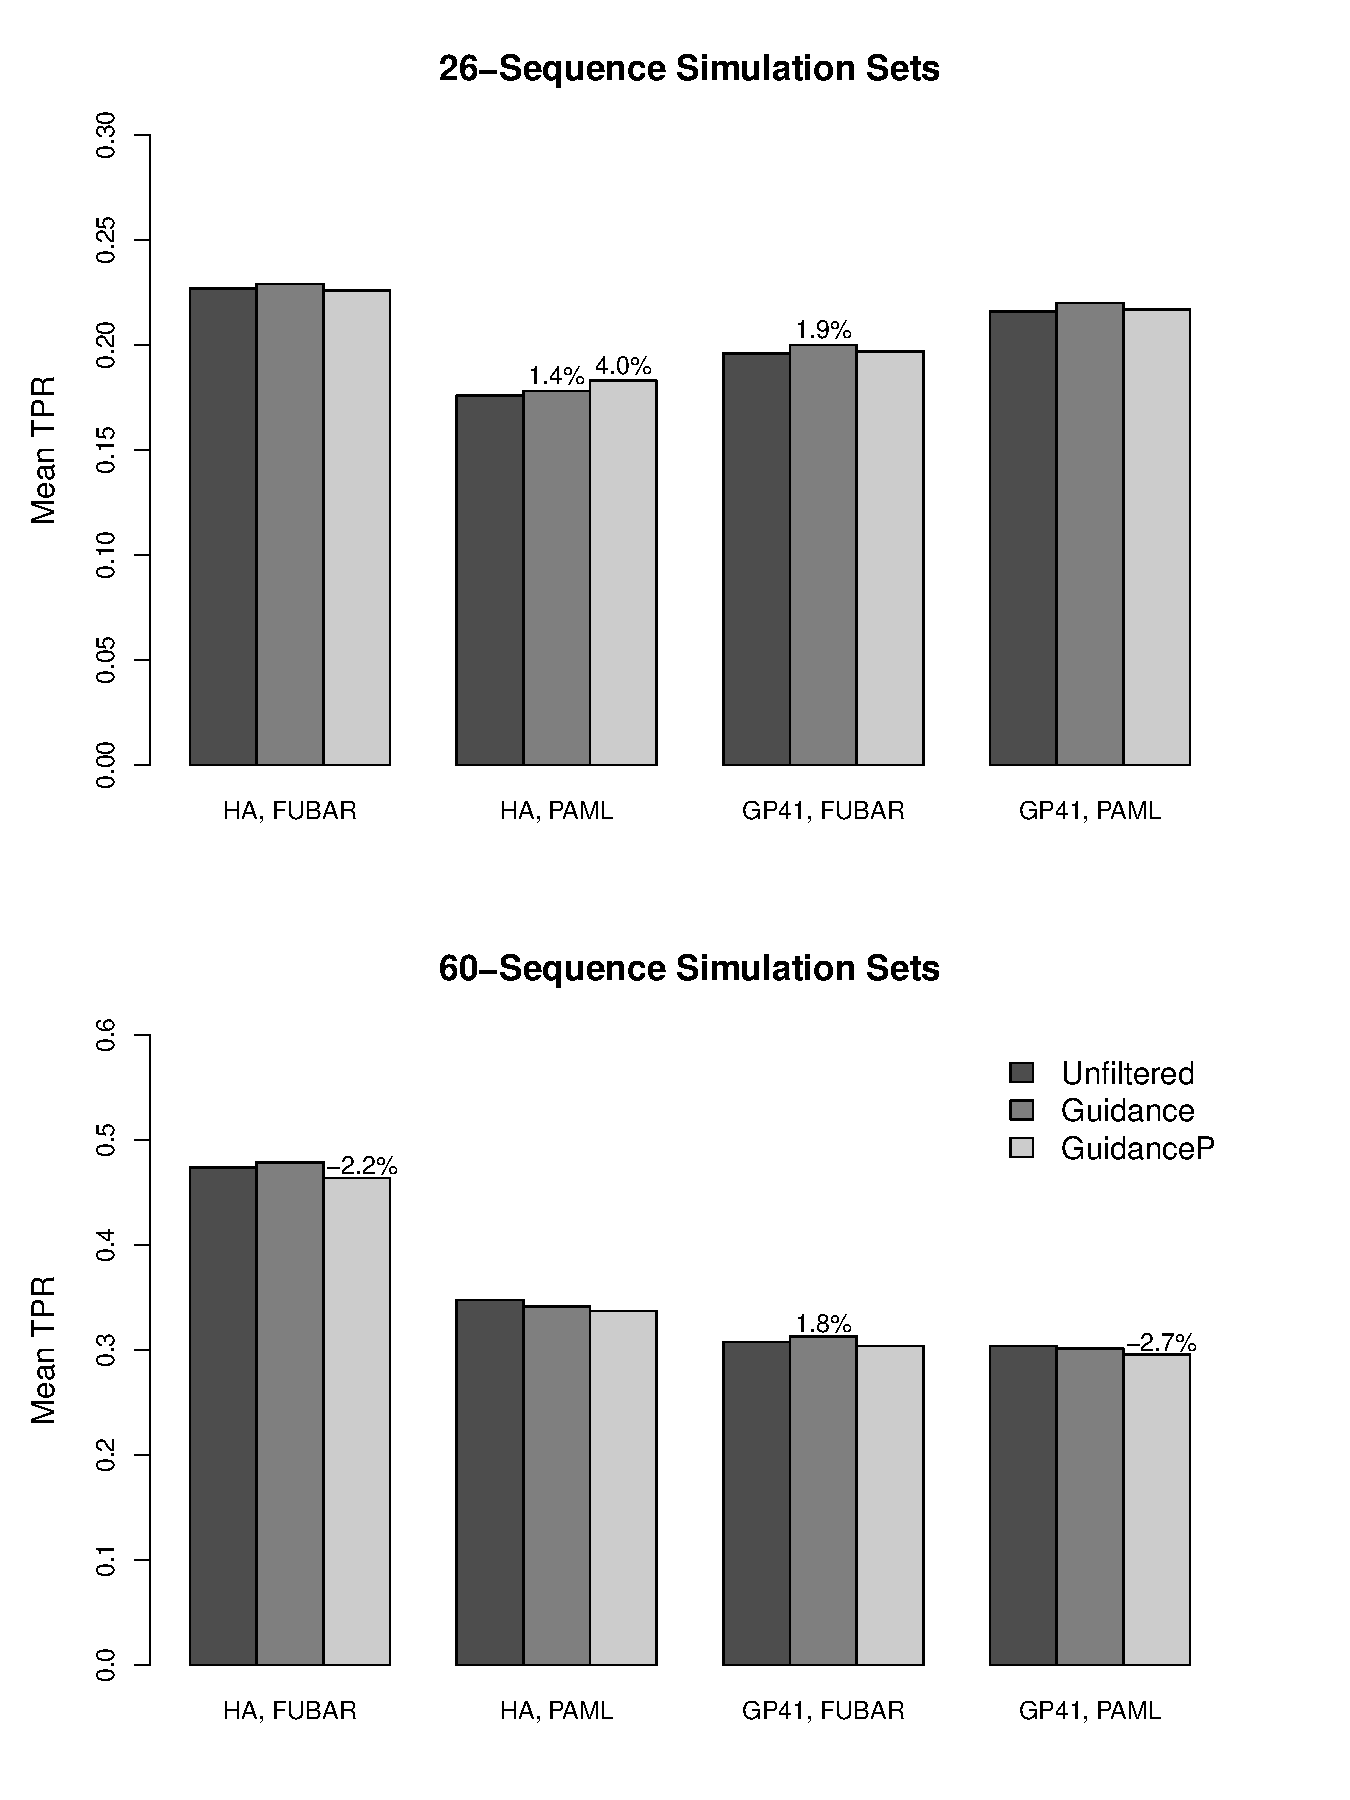
\includegraphics[width=4.75in]{Figures/barplot.pdf}}
\caption{\label{barplot} Mean TPR for and 26- and  60-sequence simulation sets. Percentages, which represent the average percent TPR change relative to the unfiltered MSAs, are shown only for those changes which are significant. Significance levels are the same as those given in Table \ref{tab:summarystats}. (A) Simulations with 26 sequences. (B) Simulations with 60 sequences.}
\end{figure*}

\bigskip

\begin{figure*}[H]
\centerline{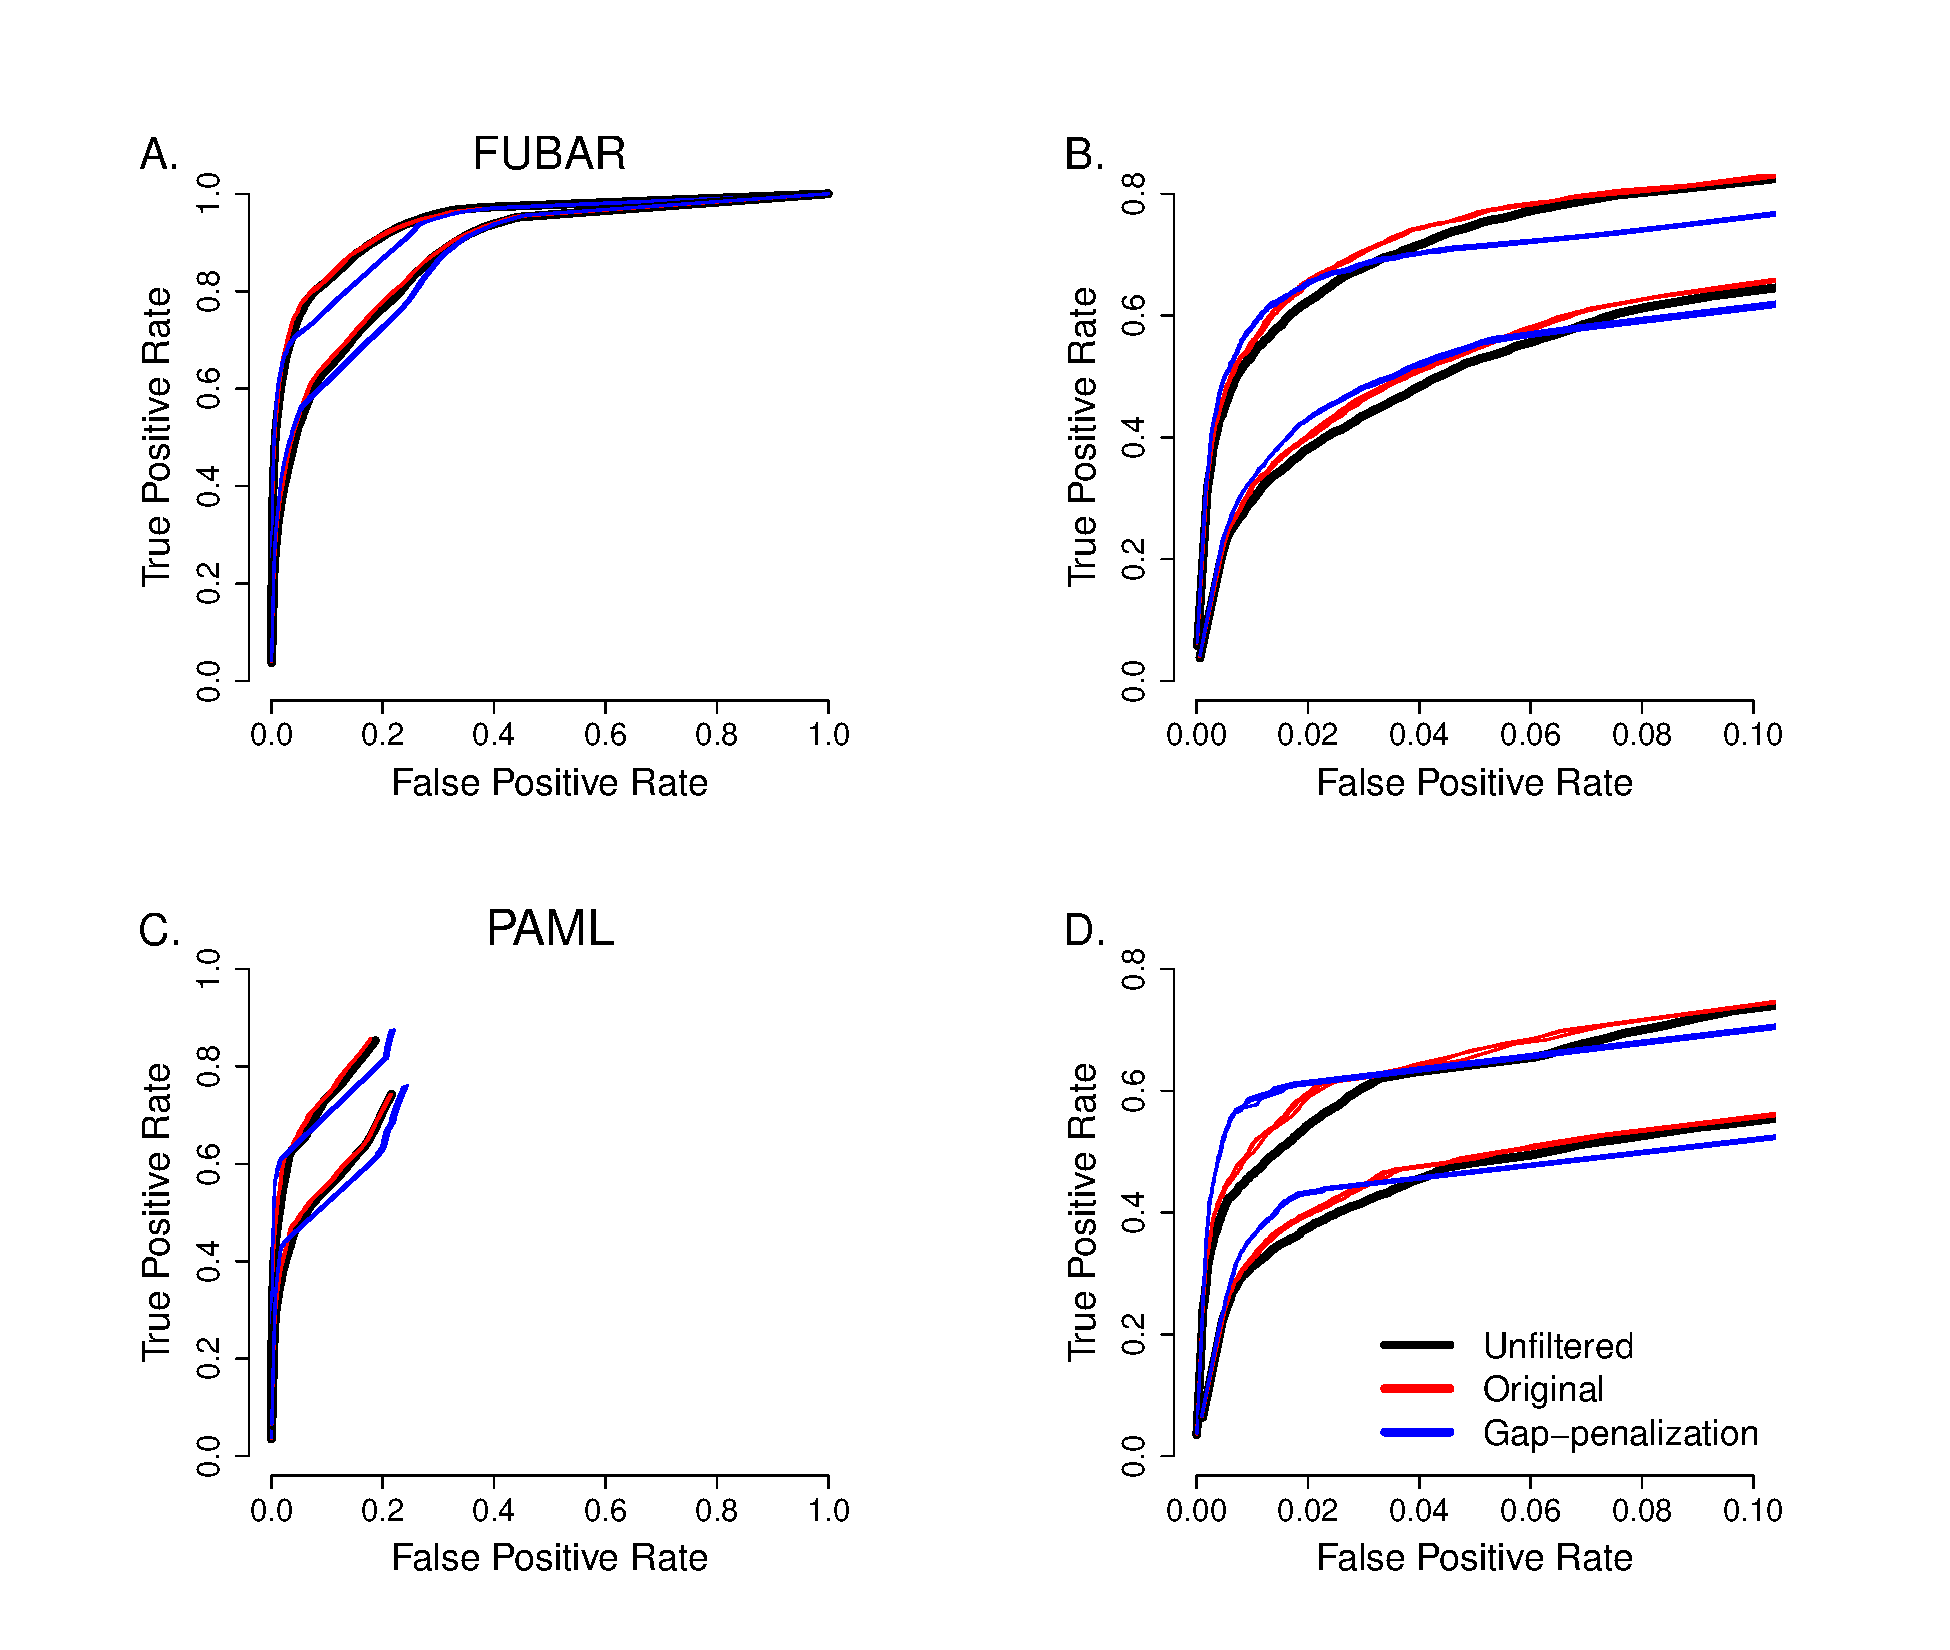
\includegraphics[width=6in]{Figures/ROC_prk.pdf}}
\caption{\label{roc} ROC curves as averaged across the two 60-sequence simulation sets. Within each panel, the top curve represents results from the HA selective profile, and the bottom curve represents results from the GP41 selective profile. Full ROC curves are shown in the left-hand panels. Note that, for the full PAML ROC curves, average FPRs higher than shown were not seen. The right-hand panels highlight specifically the low FPR regions ($0-0.1$) of the ROC curves. All MSA filtering algorithms (Guidance, BMweights, PDweights, GuidanceP, BMweightsP, and PDweightsP) are shown in ROC curves. (A,B) ROC curves for positive-selection inference by FUBAR. (C,D) ROC curves for positive-selection inference by PAML M8.}
\end{figure*}

\end{document}